\documentclass[11pt,a4paper]{article}
\usepackage[margin=2.5cm]{geometry}
\usepackage[T1]{fontenc}
\usepackage{mathptmx}
\usepackage[expansion=false]{microtype}
\usepackage{amsmath,amssymb}
\usepackage{booktabs}
\usepackage{graphicx}
\usepackage{xcolor}
\usepackage[numbers,sort&compress]{natbib}
\usepackage[colorlinks=true,linkcolor=blue!50!black,citecolor=blue!50!black,urlcolor=blue!50!black]{hyperref}
\newcommand{\nDev}{328}
\newcommand{\nTest}{768}
\newcommand{\nTasks}{1096}
\newcommand{\tunedSim}{0.8}
\newcommand{\tunedTrust}{0.0}
\newcommand{\tunedEv}{0.1}
\newcommand{\tunedStale}{0.05}
\newcommand{\tunedHL}{365}
\newcommand{\devMRR}{0.693}
\newcommand{\devHit}{0.823}
\newcommand{\gridSize}{420}
\newcommand{\hitFiveSnap}{0.641}
\newcommand{\hitOneSnap}{0.378}
\newcommand{\mrrSnap}{0.497}
\newcommand{\hitFiveEmv}{0.684}
\newcommand{\hitOneEmv}{0.406}
\newcommand{\mrrEmv}{0.532}
\newcommand{\hitFiveTuned}{0.751}
\newcommand{\hitOneTuned}{0.454}
\newcommand{\mrrTuned}{0.585}
\newcommand{\hitFivePlain}{0.551}
\newcommand{\hitOnePlain}{0.333}
\newcommand{\mrrPlain}{0.433}
\newcommand{\hitFiveNaive}{0.612}
\newcommand{\hitOneNaive}{0.357}
\newcommand{\mrrNaive}{0.470}
\newcommand{\hitFivePop}{0.451}
\newcommand{\hitOnePop}{0.083}
\newcommand{\mrrPop}{0.244}
\newcommand{\hitFiveRec}{0.451}
\newcommand{\hitOneRec}{0.189}
\newcommand{\mrrRec}{0.307}
\newcommand{\deadPlain}{0.179}
\newcommand{\deadNaive}{0.181}
\newcommand{\deadBlind}{0.015}
\newcommand{\contamPlain}{0.267}
\newcommand{\deadShare}{20}
\newcommand{\plainDeadTasks}{54}
\newcommand{\shufSnapFive}{0.130}
\newcommand{\shufEmvFive}{0.461}
\newcommand{\leakSnapOne}{0.999}
\newcommand{\leakEmvOne}{0.999}
\newcommand{\trustMean}{1.000}
\newcommand{\trustECE}{0.594}
\newcommand{\aurocGapEmv}{0.751}
\newcommand{\aurocGapSnap}{0.820}
\newcommand{\aurocGapTuned}{0.783}
\newcommand{\aurocTrustEmv}{0.500}
\newcommand{\covTwentyEmv}{0.3}
\newcommand{\accTwentyEmv}{100.0}
\newcommand{\covTwentyTuned}{5.1}
\newcommand{\accTwentyTuned}{97.4}
\newcommand{\covTwentySnap}{6.2}
\newcommand{\accTwentySnap}{93.8}
\newcommand{\covTenEmv}{5.7}
\newcommand{\accTenEmv}{93.2}
\newcommand{\covTenTuned}{14.3}
\newcommand{\accTenTuned}{92.7}
\newcommand{\covTenSnap}{16.7}
\newcommand{\accTenSnap}{88.3}
\newcommand{\covFiveEmv}{15.9}
\newcommand{\accFiveEmv}{86.1}
\newcommand{\covFiveTuned}{29.6}
\newcommand{\accFiveTuned}{82.8}
\newcommand{\covFiveSnap}{31.5}
\newcommand{\accFiveSnap}{74.8}
\newcommand{\dTunedSnapFive}{0.111}
\newcommand{\dTunedSnapLo}{0.082}
\newcommand{\dTunedSnapHi}{0.142}
\newcommand{\tunedOnly}{117}
\newcommand{\snapOnly}{32}
\newcommand{\dEmvSnapFive}{0.043}
\newcommand{\dEmvSnapLo}{0.000}
\newcommand{\dEmvSnapHi}{0.086}
\newcommand{\pEmvSnap}{0.112}
\newcommand{\dEmvPlainFive}{0.133}
\newcommand{\dEmvPlainLo}{0.090}
\newcommand{\dEmvPlainHi}{0.176}
\newcommand{\dTunedEmvFive}{0.068}
\newcommand{\dTunedEmvLo}{0.038}
\newcommand{\dTunedEmvHi}{0.100}
\newcommand{\dTunedSnapOne}{0.077}
\newcommand{\dSnapPlainFive}{0.090}
\newcommand{\ablNoTrust}{+0.021}
\newcommand{\ablNoStale}{+0.035}
\newcommand{\repFastSnap}{0.541}
\newcommand{\repFastEmv}{0.645}
\newcommand{\repFastTuned}{0.715}
\newcommand{\repFastPop}{0.640}
\newcommand{\repFastPlain}{0.384}
\newcommand{\repYtdlpSnap}{0.801}
\newcommand{\repYtdlpEmv}{0.689}
\newcommand{\repYtdlpTuned}{0.893}
\newcommand{\repYtdlpPop}{0.260}
\newcommand{\repYtdlpPlain}{0.796}
\newcommand{\repBuSnap}{0.605}
\newcommand{\repBuEmv}{0.698}
\newcommand{\repBuTuned}{0.698}
\newcommand{\repBuPop}{0.463}
\newcommand{\repBuPlain}{0.502}
\newcommand{\nClaims}{1750}

\graphicspath{{figures/}}
\setlength{\parskip}{0.4em}
\newcommand{\sys}{EmemoVeri}

\title{Evidence-Aware Memory for Coding Agents on Real Repository History:\\ A Leakage-Controlled Evaluation}
\author{Mihit\\ \small IILM University, Greater Noida, India}
\date{}

\begin{document}
\maketitle

\begin{abstract}
Coding agents that keep memory about a repository must cope with knowledge that goes stale, is contradicted, or was never reliable. We study \sys{}, a memory mechanism that attaches typed, timestamped evidence to repository claims, evolves a claim state (provisional, corroborated, refined, contested, superseded), maintains a trust value, and ranks claims with an evidence-, staleness- and scope-aware score. Earlier evaluations of this design relied on simulated scenarios whose generator shares structure with the scoring function, so they cannot support real-world claims. We replace them with a benchmark that replays the git history of three open-source repositories (fastapi, yt-dlp, browser-use) on one chronological clock and asks a memory system to rank the files that a \emph{future} commit will modify, given only its subject line and memory built from strictly earlier history. Reference files come from git, relations between commits and claims come from structural events (add, modify, delete, rename, revert) rather than keywords, and the harness includes a leak canary, a shuffled-query control, and a strict dev/test split in time. On \nTest{} held-out tasks, a dev-tuned \sys{} configuration improves Hit@5 over a snapshot-aware similarity baseline by \dTunedSnapFive{} (95\% CI [\dTunedSnapLo{}, \dTunedSnapHi{}]), and state-aware retrieval removes the dead-path suggestions (\deadPlain{} of top-5 slots) that unfiltered retrieval produces. The picture is less favourable for parts of the original design: with the blueprint weights the gain over snapshot retrieval is small and not significant after correction (\dEmvSnapFive{}, Holm $p=\pEmvSnap{}$), the trust term is saturated and uninformative, the tuner sets its weight to about zero, and the abstention rule is no better than a plain similarity gap. We release the code, tests, and all result files, and document eight defects that we found and fixed in the original implementation.
\end{abstract}

\section{Introduction}
A coding agent that works on the same repository over weeks accumulates knowledge: which module owns a behaviour, which API replaced a deprecated one, which test guards an invariant. Such knowledge decays. Files are renamed or deleted, changes are reverted, and conclusions drawn from one commit are overturned by the next. A memory that simply stores and retrieves text treats an outdated statement and a current one alike. \sys{} is a design that tries to address this by tracking \emph{evidence} for each remembered claim and letting the claim's \emph{state} change as evidence arrives.

The design is easy to describe and hard to evaluate honestly. Real tasks require a model in the loop, long runs, and labels that do not depend on the memory under test. Synthetic scenarios are cheap, but when the scenario generator decides which claim is correct by giving it higher trust, fresher timestamps and test evidence, it rewards exactly the features the scorer uses. We found that this was true of the original \sys{} experiments, and we do not use them as evidence here.

This paper makes four contributions.
\begin{enumerate}
\item \textbf{A leakage-controlled replay benchmark on real history.} Memory is built commit by commit on a single chronological clock; every task is scored before its own commit is ingested; relations come from structural git events; reference files come from git. Section~\ref{sec:bench} describes the construction, a leak canary that verifies the harness detects leakage, and a shuffled-query control that quantifies how much of a score is independent of the query.
\item \textbf{A comparison against baselines that matter.} Besides plain and naive retrieval we include \emph{snapshot RAG}, a similarity baseline that discards files absent from the current checkout. This is what an agent with a working tree obtains at no cost, and it absorbs most of the benefit of knowing that a file is gone.
\item \textbf{A component analysis with null results reported.} We ablate the trust, evidence, staleness, state and cross-repository components, evaluate selective answering, and report where the original design does not help.
\item \textbf{An audit of the original implementation.} Eight defects, including a leakage guard that leaked, a supersession state that was not terminal, and retrieval that ignored claim state, are documented, fixed, and covered by regression tests.
\end{enumerate}
We do not claim that \sys{} improves end-to-end agent success; no language model is in the loop. We claim only what the benchmark measures: how well a memory mechanism localises future changes from earlier history, and what each component contributes to that.

\section{Related work}
\textbf{Memory for language-model agents.} Retrieval-augmented generation~\cite{lewis2020rag} grounds generation in retrieved text. Agent-memory systems add write and update policies: MemGPT manages a tiered context~\cite{packer2023memgpt}, Generative Agents retrieve by recency, importance and relevance~\cite{park2023generative}, Reflexion stores verbal feedback across trials~\cite{shinn2023reflexion}, and recent systems such as Mem0~\cite{chhikara2025mem0} and A-MEM~\cite{xu2025amem} organise and update memories dynamically. LongMemEval measures long-term memory abilities of chat assistants, including knowledge updates~\cite{wu2024longmemeval}. Our setting differs in that the memory is about a code repository, updates come from version-control events, and the ground truth can be read from the history itself.

\textbf{Repository-level code assistance.} SWE-bench evaluates agents on real issues~\cite{jimenez2024swebench}, SWE-agent studies agent--computer interfaces~\cite{yang2024sweagent}, and RepoCoder retrieves repository context iteratively for completion~\cite{zhang2023repocoder}. These evaluate task success with a model in the loop. We evaluate a memory component in isolation, at lower cost and lower realism.

\textbf{Mining software repositories.} Using change history to guide edits has a long record: co-change mining suggests related files~\cite{zimmermann2005mining}, cached history and code-change complexity predict where faults occur~\cite{kim2007cache,hassan2009complexity}, and information-retrieval bug localisation ranks files against a report~\cite{zhou2012buglocator}. A recurring lesson, which our results echo, is that simple activity priors such as recency and change frequency are strong. Common pitfalls of repository mining are discussed by Kalliamvakou et al.~\cite{kalliamvakou2014perils}. We read history with plain \texttt{git} in the spirit of tools such as PyDriller~\cite{spadini2018pydriller}.

\textbf{Selective prediction and calibration.} Answering only when confident is studied as selective classification~\cite{geifman2017selective}; calibration is commonly summarised by expected calibration error~\cite{guo2017calibration}. We use both to assess the trust value and the abstention rule.

\section{The \sys{} mechanism}
\label{sec:mech}
\textbf{Claims and evidence.} A claim has a statement, a scope, a state, and a trust value in $[0,1]$. Evidence items have a type (commit, test, issue, documentation, agent observation, external), a relation to the claim (corroborates, refines, contradicts, supersedes), a timestamp, and a strength. Each type has a reliability prior, and each relation has a sign.

\textbf{State.} A claim starts PROVISIONAL and moves to CORROBORATED, REFINED or CONTESTED as evidence accumulates. SUPERSEDED is terminal: later evidence is recorded for provenance but cannot revive the claim. (In the original implementation this was not the case; see Section~\ref{sec:audit}.)

\textbf{Trust.} The default update is sequential and clamped, $t \leftarrow \mathrm{clip}(t + \eta\, w_e,0,1)$ with learning rate $\eta=0.35$. We also implement a pooled clamped update and an order-invariant, non-saturating update, $t=\sigma(\mathrm{logit}(t_0)+\eta\sum_e w_e)$.

\textbf{Retrieval score.} For a query with scope $q$ at reference time $\tau$,
\begin{equation}
s = 0.45\,\mathrm{sim} + 0.25\,\mathrm{trust} + 0.20\,\mathrm{evid} + 0.10\,\mathrm{scope} - 0.10\,\mathrm{stale},
\end{equation}
where $\mathrm{evid}=E/(E+5)$ for total evidence strength $E$, $\mathrm{stale}=1-2^{-\Delta/H}$ with $\Delta$ the time since the last update and $H=90$ days, and $\mathrm{scope}$ is 1 for a same-scope claim and 0 otherwise. SUPERSEDED claims are excluded. A local-first policy admits a cross-scope claim only if its score exceeds the best local score by a margin.

\textbf{Abstention.} A conflict resolver answers with the top claim when the score gap to the runner-up is at least $0.20$, and abstains otherwise.

\section{Benchmark}
\label{sec:bench}
\subsection{Task}
At time $t$ the system receives the cleaned subject line of a \emph{future} commit $C$ and must rank source files. Memory contains only information from commits strictly before $C$. The reference set is the set of source files that $C$ modified. No classifier is involved in producing it. Because the query is the subject of a commit that has not yet happened, it stands in for a task description; it is more specific than a typical issue and we return to this in Section~\ref{sec:threats}.

\subsection{Memory from structural events}
There is one claim per live \texttt{.py} file under the repository's source root. Relations are read from git's own status letters rather than inferred from wording: an addition corroborates, a modification refines, a deletion or a rename away supersedes, and a commit carrying git's ``This reverts commit'' trailer contradicts the claims of the files it touches. A rename carries the file's evidence and text to the new path and supersedes the old claim; a path that reappears after deletion becomes a new claim. Evidence is of type TEST when the commit also edits a test file and COMMIT otherwise, with strength 1.0, or 0.3 for bulk commits that touch more than three source files. Claim text is the file path plus the five most recent cleaned subjects of commits touching it. Similarity is cosine over hashed unigram and bigram TF-IDF vectors in which IDF is recomputed from pre-cutoff claims for every task, so no statistic is fitted on later data.

Commits are replayed in topological order. Real histories contain non-monotone timestamps (Table~\ref{tab:data}), so the clock is the running maximum of committer timestamps. Table~\ref{tab:events} shows how often each structural event occurs: deletions and renames are common in yt-dlp, but reverts that touch source files are rare, so the contradiction path is exercised only lightly.

\begin{table}[t]\centering\small
\resizebox{\linewidth}{!}{\begin{tabular}{lrrrrrr}
\toprule
Repository & Commits & Source-touching & Eligible & Selected & Cold-file excl. & Clock anomalies \\
\midrule
fastapi & 7,712 & 853 & 296 & 296 & 0 & 12 \\
yt-dlp & 22,449 & 5,052 & 1,885 & 400 & 0 & 2,289 \\
browser-use & 7,003 & 4,057 & 1,773 & 400 & 5 & 4,294 \\
\bottomrule
\end{tabular}}
\caption{Mined repositories and task selection. ``Eligible'' tasks are non-bot, non-revert, modify one to four source files that already have a claim, and occur after a warm-up of 35\% of the repository's source-touching commits; up to 400 evenly spaced tasks per repository are selected. Clock anomalies are commits whose recorded timestamp precedes the running clock. History of yt-dlp that predates its \texttt{yt\_dlp/} package directory is outside the source root and therefore not tracked.}
\label{tab:data}
\end{table}

\begin{table}[t]\centering\small
\resizebox{\linewidth}{!}{\begin{tabular}{lrrrrr}
\toprule
Repository & Adds & Modifications & Deletions & Renames & Reverts (touching source) \\
\midrule
fastapi & 59 & 1,476 & 7 & 1 & 4 (3) \\
yt-dlp & 528 & 12,324 & 327 & 853 & 51 (5) \\
browser-use & 258 & 6,651 & 103 & 47 & 20 (15) \\
\bottomrule
\end{tabular}}
\caption{Structural events on source files in the full histories.}
\label{tab:events}
\end{table}

\subsection{Integrity controls}
Memory is updated only after a task has been scored, and a runtime assertion rejects any memory state containing evidence newer than the task. As a \emph{leak canary}, each task is re-scored after its own commit has been ingested; a harness that can detect leakage must show a large jump, and ours does (Hit@1 \leakSnapOne{} for snapshot RAG and \leakEmvOne{} for \sys{}). As a \emph{shuffled-query control}, each task is scored with another task's query. Weights are tuned only on the earliest 30\% of tasks on the global clock (\nDev{} dev tasks, \nTest{} test tasks); a \gridSize{}-point grid over similarity, trust and evidence weights, staleness weight and half-life, and trust update mode is searched by dev MRR. browser-use appears only in the test period, so it serves as a repository unseen during tuning.

\subsection{Conditions and metrics}
\textbf{Query-independent priors:} random live file, most recently updated, most evidence. \textbf{Plain RAG:} similarity only, over all repositories, dead files included. \textbf{Naive memory:} similarity only, local repository, dead files included. \textbf{Snapshot RAG:} similarity only, local repository, dead files removed. \textbf{\sys{}:} the score above with blueprint weights. \textbf{\sys{} tuned:} dev-selected weights. We report Hit@$k$ (a reference file among the top $k$ distinct files), MRR, the fraction of top-5 slots that are dead paths, and the fraction that come from another repository. Differences are paired at task level with 10{,}000-sample bootstrap intervals; binary outcomes use an exact McNemar test with Holm correction over the 16 binary comparisons.

\section{Results}
\subsection{Comparison with baselines}
Table~\ref{tab:main} and Figure~\ref{fig:main} give test-set results. Unfiltered retrieval suffers from two hazards that are easy to measure here. Plain RAG places a file from another repository in \contamPlain{} of its top-5 slots, and both plain RAG and naive memory place a deleted or renamed-away path in about \deadPlain{} of them; at query time about \deadShare{}\% of all claims are dead, and \plainDeadTasks{}\% of test tasks have at least one dead path in the plain-RAG top five. Removing dead files alone (snapshot RAG) raises Hit@5 by \dSnapPlainFive{} over plain RAG (Figure~\ref{fig:haz}).

\begin{table}[t]\centering\small
\resizebox{\linewidth}{!}{\begin{tabular}{lcccccc}
\toprule
Condition & Hit@1 & Hit@3 & Hit@5 & MRR & Dead@5 & Other-repo@5 \\
\midrule
Random (local) & 0.016 & 0.047 & 0.081 & 0.051 & 0.000 & 0.000 \\
Recency & 0.189 & 0.375 & 0.451 & 0.307 & 0.000 & 0.000 \\
Popularity & 0.083 & 0.371 & 0.451 & 0.244 & 0.000 & 0.000 \\
\midrule
Plain RAG (all repos) & 0.333 & 0.495 & 0.551 & 0.433 & 0.179 & 0.267 \\
Naive memory (local) & 0.357 & 0.531 & 0.612 & 0.470 & 0.181 & 0.000 \\
\midrule
Snapshot RAG & 0.378 & 0.564 & 0.641 & 0.497 & 0.000 & 0.000 \\
\midrule
EmemoVeri (default weights) & 0.406 & 0.607 & 0.684 & 0.532 & 0.000 & 0.000 \\
EmemoVeri (dev-tuned) & 0.454 & 0.661 & 0.751 & 0.585 & 0.000 & 0.000 \\
\bottomrule
\end{tabular}}
\caption{Test results ($n=\nTest{}$). Dead@5 and Other-repo@5 are the fractions of top-5 slots that are dead paths or files from another repository.}
\label{tab:main}
\end{table}

\begin{figure}[t]\centering
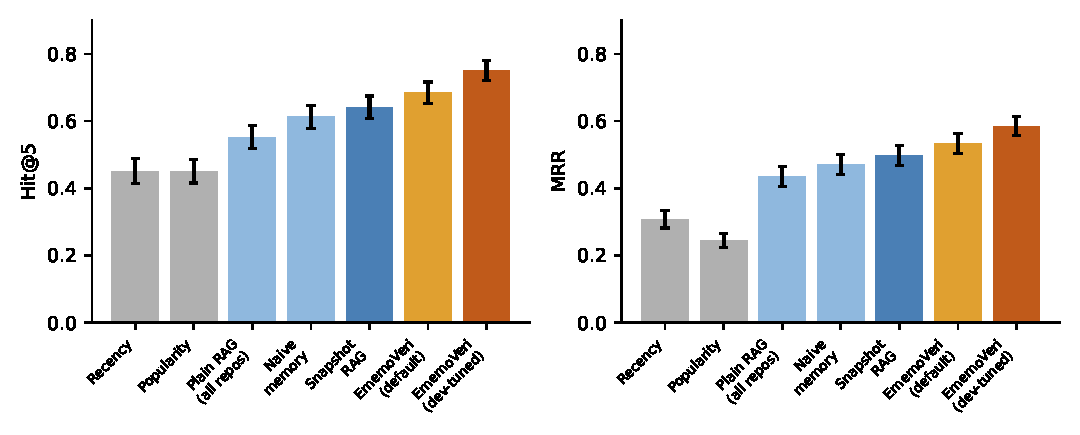
\includegraphics[width=0.95\linewidth]{fig_main.pdf}
\caption{Hit@5 and MRR on the test split with 95\% bootstrap intervals.}
\label{fig:main}
\end{figure}

With the blueprint weights, \sys{} improves Hit@5 over plain RAG by \dEmvPlainFive{} (95\% CI [\dEmvPlainLo{}, \dEmvPlainHi{}]) but over snapshot RAG by only \dEmvSnapFive{} (95\% CI [\dEmvSnapLo{}, \dEmvSnapHi{}], Holm $p=\pEmvSnap{}$), which is not significant after correction (Table~\ref{tab:cmp}). Most of what state-aware memory offers over naive retrieval is therefore available to any agent that can see its working tree. The dev-tuned configuration, in contrast, improves Hit@5 over snapshot RAG by \dTunedSnapFive{} (95\% CI [\dTunedSnapLo{}, \dTunedSnapHi{}]); on \tunedOnly{} tasks only the tuned system hits and on \snapOnly{} only snapshot RAG hits. The selected weights are \tunedSim{} similarity, \tunedTrust{} trust, \tunedEv{} evidence, \tunedStale{} staleness (half-life \tunedHL{} days): a mostly lexical ranker with a light activity prior.

\begin{table}[t]\centering\small
\resizebox{\linewidth}{!}{\begin{tabular}{llcccc}
\toprule
A & B & Metric & $\Delta$ (A$-$B) [95\% CI] & A-only / B-only & $p_{\text{Holm}}$ \\
\midrule
EmemoVeri (default weights) & Plain RAG (all repos) & Hit@1 & +0.073 [+0.036, +0.109] & 132 / 76 & 0.0008 \\
EmemoVeri (default weights) & Plain RAG (all repos) & Hit@5 & +0.133 [+0.090, +0.176] & 203 / 101 & $<$0.0001 \\
\midrule
EmemoVeri (default weights) & Naive memory (local) & Hit@1 & +0.049 [+0.013, +0.086] & 121 / 83 & 0.0282 \\
EmemoVeri (default weights) & Naive memory (local) & Hit@5 & +0.072 [+0.029, +0.115] & 171 / 116 & 0.0070 \\
\midrule
EmemoVeri (default weights) & Snapshot RAG & Hit@1 & +0.029 [$-$0.009, +0.065] & 113 / 91 & 0.1413 \\
EmemoVeri (default weights) & Snapshot RAG & Hit@5 & +0.043 [+0.000, +0.086] & 157 / 124 & 0.1121 \\
\midrule
EmemoVeri (dev-tuned) & Snapshot RAG & Hit@1 & +0.077 [+0.052, +0.103] & 82 / 23 & $<$0.0001 \\
EmemoVeri (dev-tuned) & Snapshot RAG & Hit@5 & +0.111 [+0.082, +0.142] & 117 / 32 & $<$0.0001 \\
\midrule
EmemoVeri (dev-tuned) & EmemoVeri (default weights) & Hit@1 & +0.048 [+0.020, +0.077] & 84 / 47 & 0.0070 \\
EmemoVeri (dev-tuned) & EmemoVeri (default weights) & Hit@5 & +0.068 [+0.038, +0.100] & 105 / 53 & 0.0003 \\
\midrule
Snapshot RAG & Plain RAG (all repos) & Hit@1 & +0.044 [+0.031, +0.060] & 34 / 0 & $<$0.0001 \\
Snapshot RAG & Plain RAG (all repos) & Hit@5 & +0.090 [+0.070, +0.111] & 69 / 0 & $<$0.0001 \\
\bottomrule
\end{tabular}}
\caption{Paired comparisons on the test split. A-only / B-only count tasks where only A or only B has a hit.}
\label{tab:cmp}
\end{table}

\subsection{Repositories differ}
Table~\ref{tab:repo} and Figure~\ref{fig:repo} break results down by repository. The default weights help on fastapi and browser-use but hurt on yt-dlp, where Hit@5 falls from \repYtdlpSnap{} (snapshot RAG) to \repYtdlpEmv{}. A likely reason, which we did not test directly, is that yt-dlp has one extractor file per website, so path tokens match queries well and a query-independent prior mostly adds noise. The tuned configuration recovers this (\repYtdlpTuned{}), and its gain holds on browser-use, which tuning never saw (\repBuSnap{} for snapshot RAG against \repBuTuned{} tuned). On fastapi, popularity alone reaches \repFastPop{}, comparable to the default \sys{} (\repFastEmv{}), because a few hot files account for most edits. Any aggregate number should be read with this heterogeneity in mind.

\begin{table}[t]\centering\small
\begin{tabular}{llccc}
\toprule
Repository ($n$) & Condition & Hit@1 & Hit@5 & MRR \\
\midrule
browser-use (400) & Popularity & 0.147 & 0.463 & 0.289 \\
 & Plain RAG (all repos) & 0.258 & 0.502 & 0.364 \\
 & Snapshot RAG & 0.315 & 0.605 & 0.442 \\
 & EmemoVeri (default weights) & 0.393 & 0.698 & 0.523 \\
 & EmemoVeri (dev-tuned) & 0.403 & 0.698 & 0.532 \\
\midrule
fastapi (172) & Popularity & 0.012 & 0.640 & 0.275 \\
 & Plain RAG (all repos) & 0.198 & 0.384 & 0.293 \\
 & Snapshot RAG & 0.244 & 0.541 & 0.387 \\
 & EmemoVeri (default weights) & 0.297 & 0.645 & 0.464 \\
 & EmemoVeri (dev-tuned) & 0.326 & 0.715 & 0.493 \\
\midrule
yt-dlp (196) & Popularity & 0.015 & 0.260 & 0.125 \\
 & Plain RAG (all repos) & 0.607 & 0.796 & 0.697 \\
 & Snapshot RAG & 0.622 & 0.801 & 0.708 \\
 & EmemoVeri (default weights) & 0.531 & 0.689 & 0.611 \\
 & EmemoVeri (dev-tuned) & 0.673 & 0.893 & 0.773 \\
\bottomrule
\end{tabular}
\caption{Test results by repository.}
\label{tab:repo}
\end{table}

\begin{figure}[t]\centering
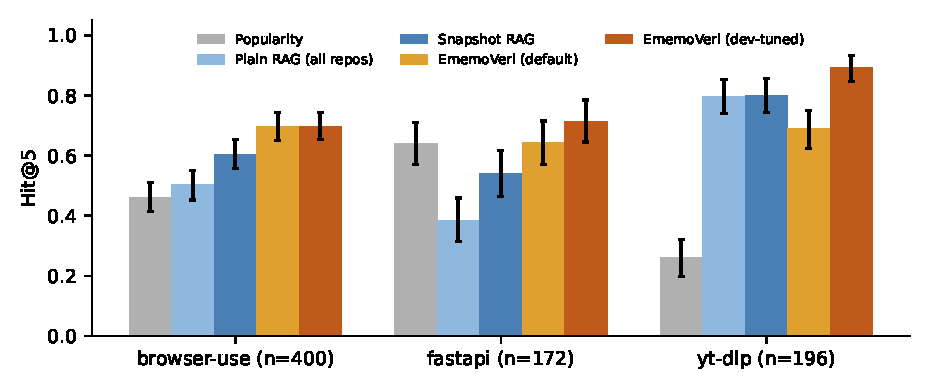
\includegraphics[width=0.8\linewidth]{fig_repo.pdf}
\caption{Hit@5 by repository with 95\% bootstrap intervals.}
\label{fig:repo}
\end{figure}

\subsection{What each component contributes}
Table~\ref{tab:abl} and Figure~\ref{fig:abl} ablate the default system. The state-aware filter does what it is designed to do for staleness: without it, \deadBlind{} of top-5 slots are dead paths instead of none, but Hit@5 barely changes because dead files are almost never reference files. Removing the trust term or the staleness term \emph{improves} Hit@5 (\ablNoTrust{} and \ablNoStale{}), a longer half-life helps, and a shorter one does not (its interval includes zero). The evidence term's effect is not distinguishable from zero. The three cross-repository policies are indistinguishable in the top five, because the scope term alone keeps other repositories out; the policy only matters if the scope weight is removed, as in plain RAG. The non-saturating trust update does not rescue the trust signal. Taken together, the gain of the tuned system over the default comes mostly from down-weighting trust and staleness and keeping a small evidence prior.

\begin{table}[t]\centering\small
\resizebox{\linewidth}{!}{\begin{tabular}{lcc}
\toprule
Variant of default EmemoVeri & $\Delta$Hit@5 [95\% CI] & $\Delta$MRR [95\% CI] \\
\midrule
No trust term & +0.021 [+0.010, +0.033] & +0.007 [+0.001, +0.013] \\
No evidence term & $-$0.012 [$-$0.047, +0.023] & +0.009 [$-$0.016, +0.033] \\
No staleness term & +0.035 [+0.018, +0.052] & +0.023 [+0.011, +0.037] \\
State-blind (keep SUPERSEDED) & $-$0.001 [$-$0.004, +0.000] & $-$0.003 [$-$0.005, $-$0.001] \\
Cross-repo: open & +0.000 [+0.000, +0.000] & $-$0.000 [$-$0.001, $-$0.000] \\
Cross-repo: local only & +0.000 [+0.000, +0.000] & +0.000 [+0.000, +0.000] \\
Cross-repo: similarity gate & +0.000 [+0.000, +0.000] & +0.000 [+0.000, +0.000] \\
Trust: pooled, clamped & +0.004 [+0.000, +0.009] & +0.002 [$-$0.001, +0.006] \\
Trust: pooled, logit & $-$0.007 [$-$0.016, +0.003] & $-$0.009 [$-$0.016, $-$0.003] \\
Staleness half-life 30 d & $-$0.013 [$-$0.027, +0.001] & $-$0.017 [$-$0.027, $-$0.008] \\
Staleness half-life 365 d & +0.016 [+0.003, +0.029] & +0.013 [+0.004, +0.022] \\
\bottomrule
\end{tabular}}
\caption{Ablations relative to default \sys{} on the test split. Positive values mean the variant is better than the default.}
\label{tab:abl}
\end{table}

\begin{figure}[t]\centering
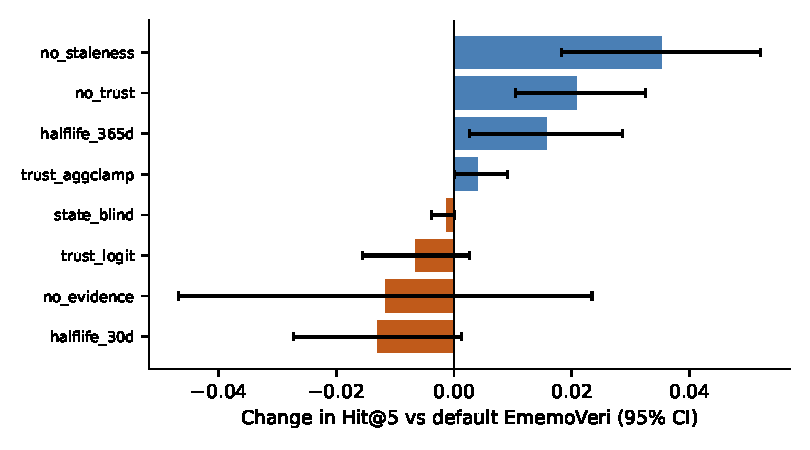
\includegraphics[width=0.75\linewidth]{fig_ablation.pdf}
\caption{Change in Hit@5 relative to default \sys{} (95\% bootstrap intervals).}
\label{fig:abl}
\end{figure}

\subsection{Trust and abstention}
For the top-ranked claim, mean trust is \trustMean{} under the default update: trust saturates, and its AUROC for predicting a correct top-1 answer is \aurocTrustEmv{}, no better than chance. Its expected calibration error (\trustECE{}) equals one minus accuracy, as expected of a constant near 1. The score gap used by the conflict resolver is informative (AUROC \aurocGapEmv{} default, \aurocGapTuned{} tuned), but a plain similarity gap on snapshot RAG is at least as good (\aurocGapSnap{}). At the prescribed threshold of 0.20 the default system answers \covTwentyEmv{}\% of tasks (\accTwentyEmv{}\% correct); the tuned system answers \covTwentyTuned{}\% (\accTwentyTuned{}\%); snapshot RAG answers \covTwentySnap{}\% (\accTwentySnap{}\%). Lower thresholds trade coverage for accuracy along a curve that is similar across systems (Figure~\ref{fig:sel}, Table~\ref{tab:sel}). We therefore find no evidence that \sys{}'s abstention rule adds value over a similarity gap in this setting.

\begin{table}[t]\centering\small
\resizebox{\linewidth}{!}{\begin{tabular}{lcccc}
\toprule
System & Top-1 acc. & AURC (gap) $\downarrow$ & AUROC (gap) & AUROC (trust) \\
\midrule
Snapshot RAG & 0.378 & 0.362 & 0.820 & 0.570 \\
EmemoVeri (default weights) & 0.406 & 0.376 & 0.751 & 0.500 \\
EmemoVeri (dev-tuned) & 0.454 & 0.307 & 0.783 & 0.489 \\
\bottomrule
\end{tabular}}
\caption{Selective answering on the top-1 file. AURC is the mean risk over coverage (lower is better); the random-confidence value equals one minus top-1 accuracy.}
\label{tab:sel}
\end{table}

\begin{figure}[t]\centering
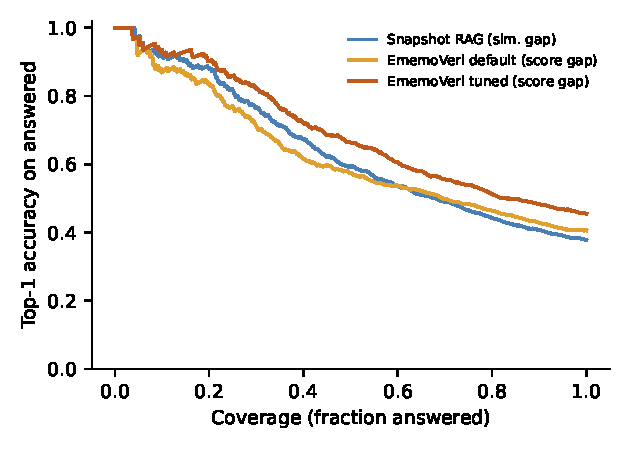
\includegraphics[width=0.6\linewidth]{fig_selective.pdf}
\caption{Top-1 accuracy among answered tasks as coverage increases, ordering by score gap.}
\label{fig:sel}
\end{figure}

\subsection{Harness validity and robustness}
The leak canary reaches Hit@1 above \leakSnapOne{}, so a leaking pipeline would be caught. The shuffled-query control is informative in the other direction: with another task's query, snapshot RAG falls to Hit@5 \shufSnapFive{}, but default \sys{} keeps \shufEmvFive{}, about the level of recency and popularity alone (\hitFiveRec{} and \hitFivePop{}). A sizeable part of the default system's score is therefore independent of the query. This is not a flaw in itself, since activity priors are known to be strong predictors in repository mining~\cite{kim2007cache,hassan2009complexity}, but it means that credit for the gain should not be assigned to evidence semantics without further study. Table~\ref{tab:rob} repeats the main comparison with a different warm-up fraction and sample size. The conclusions hold: the tuned system beats snapshot RAG by 0.09 to 0.11 Hit@5 in every setting, the default is never significantly better than snapshot RAG after correction, and the tuner assigns the trust term a weight of at most 0.1.

\begin{table}[t]\centering\small
\resizebox{\linewidth}{!}{\begin{tabular}{lccc}
\toprule
Setting (test $n$) & Default vs.\ Snapshot RAG & Tuned vs.\ Snapshot RAG & Tuned trust weight \\
\midrule
Main: warm-up 0.35, 400/repo (768) & +0.043 [+0.000, +0.086] & +0.111 [+0.082, +0.142] & 0.0 \\
Warm-up 0.20 (839) & +0.043 [+0.001, +0.085] & +0.112 [+0.085, +0.141] & 0.0 \\
Warm-up 0.50 (712) & +0.007 [$-$0.035, +0.051] & +0.088 [+0.060, +0.118] & 0.0 \\
150 tasks/repo (315) & +0.025 [$-$0.038, +0.092] & +0.111 [+0.067, +0.159] & 0.1 \\
\bottomrule
\end{tabular}}
\caption{Hit@5 differences under alternative settings (95\% bootstrap intervals).}
\label{tab:rob}
\end{table}

\begin{figure}[t]\centering
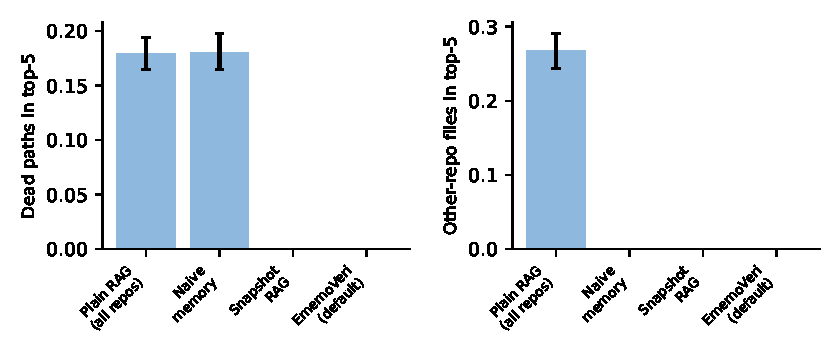
\includegraphics[width=0.85\linewidth]{fig_hazards.pdf}
\caption{Hazards of unfiltered retrieval: dead paths and other-repository files in the top five.}
\label{fig:haz}
\end{figure}

\section{Discussion}
\textbf{What is supported.} State-aware filtering removes a real and measurable class of error, suggestions of files that no longer exist, and it removes cross-repository contamination when scope is used. A tuned blend of lexical similarity with a light evidence and recency prior beats a snapshot-aware lexical baseline, consistently across settings and on a repository unseen during tuning.

\textbf{What is not.} The blueprint weights do not reliably beat snapshot retrieval; the trust value carries no usable signal under the default update, and replacing the update did not fix that; the abstention rule is not better than a similarity gap. Because the benchmark's evidence is almost all positive (modifications), it does not exercise contested states much, and we cannot say whether contradiction handling would matter in settings with more reverts or conflicting sources.

\textbf{Why the benchmark may understate or overstate.} Commit subjects are more informative than issue text, which may favour lexical similarity; real agents also see the working tree, code content and tests, which this benchmark does not use. On the other hand, the recency and popularity priors might matter more when the query is vaguer. We make no claim in either direction.

\section{Threats to validity}
\label{sec:threats}
\emph{Construct.} File localisation from a commit subject is a proxy for agent tasks; it says nothing about patch quality. \emph{Internal.} Tasks are not independent, since hot files recur and commits cluster by author and time, so bootstrap intervals over tasks are optimistic. Weights were tuned on the same task family as the test set, although in an earlier period and with one repository held out entirely. Tie-breaking favours recently updated claims, which can favour recency-heavy conditions slightly. \emph{External.} Three Python repositories, one of which has an unusual one-file-per-site layout. Results depend on the clone date; we pin repository heads in the release. \emph{Conclusion.} Sixteen binary comparisons were corrected with Holm's method; the bootstrap intervals for paired differences are not corrected.

\section{Audit of the original implementation}
\label{sec:audit}
While building the benchmark we reproduced and fixed eight defects in the first version of the code. (1) SUPERSEDED was not terminal: a later corroboration moved a superseded claim back to CORROBORATED. (2) Retrieval ignored claim state, so a superseded claim with higher trust could rank first. (3) The temporal leakage guard dropped future evidence but kept the trust and state that had been derived from it; it now replays visible evidence through the trust model and state engine. (4) Staleness defaulted to the wall clock, making every historical claim look fully stale; it now defaults to the knowledge cutoff. (5) The keyword relation classifier mislabels ordinary commits (for example, substring matches on ``add''), so real-history relations use structural git events instead. (6) Clamped trust updates saturate after two or three strong items. (7) A single candidate always resolved, regardless of score. (8) The cross-repository split used object equality in one module and identity in another. Each fix has a regression test. Results produced before these fixes, including the original synthetic experiments, should not be reused.

\section{Conclusion}
On real repository history, a memory that knows which files have disappeared, and that blends lexical similarity with a light evidence and recency prior, localises future changes better than plain retrieval and, once tuned, better than a snapshot-aware baseline. The original design's trust and abstention components did not earn their place in this setting, and the blueprint weights over-weight priors on repositories where the query is highly informative. The natural next steps are a language model in the loop on issue-derived tasks, repositories with more contradictory history, and a trust model that uses evidence beyond counts.

\paragraph{Reproducibility.} Code, tests, raw per-task outcomes, all summaries and figures, and pinned repository heads are in the accompanying repository. \texttt{scripts/}\allowbreak\texttt{reproduce\_real.sh} regenerates every number; tables and numeric macros in this paper are produced by \texttt{paper/}\allowbreak\texttt{make\_tables.py} from \texttt{results/}\allowbreak\texttt{real/}\allowbreak\texttt{summary.json}.

\paragraph{Acknowledgments.} An AI assistant (Claude, Anthropic) assisted with the code, the experiments and the drafting of this manuscript; the authors reviewed the results and are responsible for the content.

\bibliographystyle{unsrtnat}
\bibliography{refs}

\end{document}
